\documentclass{beamer}
\usepackage{graphicx}
\usepackage{multirow}
\usepackage[utf8]{inputenc}
\usepackage[UKenglish]{babel}
\usepackage[UKenglish]{isodate}
\usepackage[style=authoryear]{biblatex}
\usepackage{tikz}
\usepackage[clock]{ifsym}
\usepackage[group-separator={,}]{siunitx}
\usetikzlibrary{positioning, shapes.arrows}

\usecolortheme{rose}
\beamertemplatenavigationsymbolsempty
\addbibresource{../dissertation/references.bib}
\author{Paulius Dilkas\\{\small Supervisors: Dr Patrick Prosser and Dr Ciaran
    McCreesh}}
\title{Algorithm Selection for Maximum Common Subgraph}
\date{23rd March 2018}
\institute{School of Computing Science\\University of Glasgow}

\begin{document}
\maketitle

\begin{frame}{The Problem: Maximum Common Subgraph}
  \begin{figure}
    \centering
  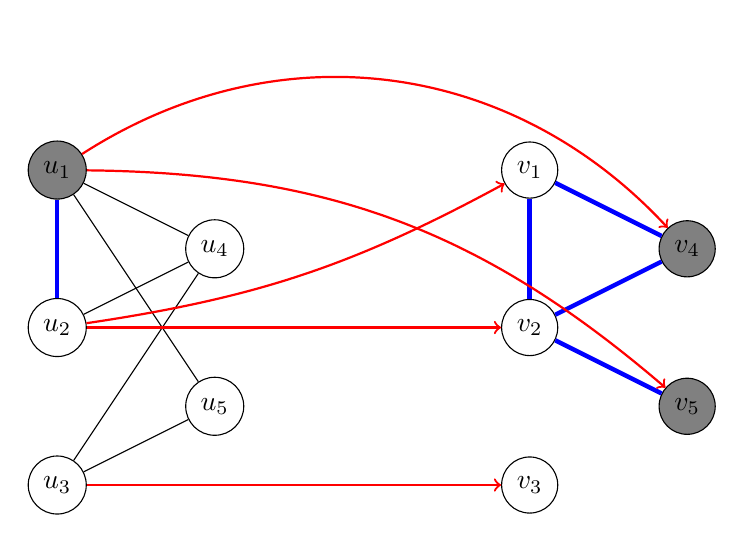
\begin{tikzpicture}
    \begin{scope}[every node/.style={circle,draw}]
      \node (u1) [fill=gray,] at (0, 4) {$u_1$};
      \node (u2) at (0, 2) {$u_2$};
      \node (u3) at (0, 0) {$u_3$};
      \node<-4> (u4) at (2, 3) {$u_4$};
      \node<-4> (u5) at (2, 1) {$u_5$};
    \end{scope}
    \path (u1) [color=blue,ultra thick] edge node {} (u2);
    \path<-4> (u1) edge node {} (u4);
    \path<-4> (u1) edge node {} (u5);
    \path<-4> (u2) edge node {} (u4);
    \path<-4> (u3) edge node {} (u4);
    \path<-4> (u3) edge node {} (u5);
    \begin{scope}[every node/.style={circle, draw},xshift=6cm]
      \node<-5> (v1) at (0, 4) {$v_1$};
      \node<-4,6-> (v2) at (0, 2) {$v_2$};
      \node (v3) at (0, 0) {$v_3$};
      \node<-6> (v4) [fill=gray] at (2, 3) {$v_4$};
      \node<-4,7> (v5) [fill=gray] at (2, 1) {$v_5$};
    \end{scope}
    \begin{scope}[color=blue,ultra thick]
      \path<-4> (v1) edge node {} (v2);
      \path<-5> (v1) edge node {} (v4);
      \path<-4,6> (v2) edge node {} (v4);
      \path<-4,7> (v2) edge node {} (v5);
    \end{scope}
    \begin{scope}[color=red,thick]
      \onslide<2-6>{\path[->] (u1) edge [bend left=40] (v4);}
      \onslide<2-4,7>{\path[->] (u1) edge [bend left=20] (v5);}
      \onslide<3-5>{\path[->] (u2) edge [bend right=10] (v1);}
      \onslide<3-4,6->{\path[->] (u2) edge [] (v2);}
      \onslide<4->{\path[->] (u3) edge [] (v3);}
    \end{scope}
  \end{tikzpicture}
  \end{figure}
\end{frame}

\begin{frame}{Why Is It Important?}
  \begin{columns}[t]
    \begin{column}{0.5\textwidth}
      \centering
      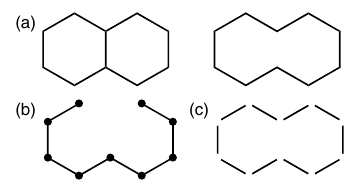
\includegraphics[width=0.9\textwidth,height=0.4\textheight,keepaspectratio]{chemistry.png} \\[-7pt]
      {\tiny Source: \cite{WCMS:WCMS5}}
      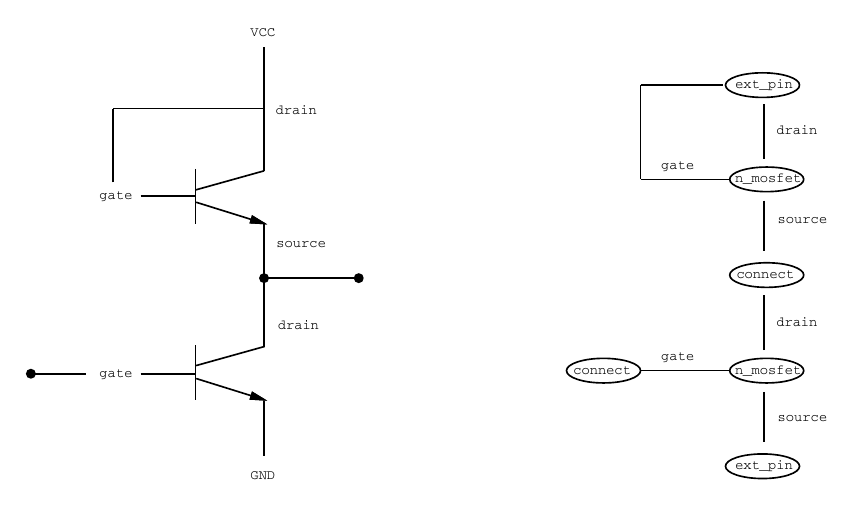
\includegraphics[width=0.9\textwidth,height=0.4\textheight,keepaspectratio]{electronics.png} \\[-7pt]
      {\tiny Source: \cite{DBLP:journals/jair/CookH94}}
    \end{column}
    \begin{column}{0.5\textwidth}
      \centering
      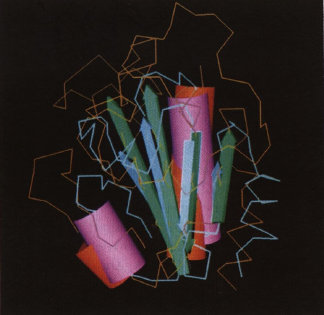
\includegraphics[width=0.9\textwidth,height=0.4\textheight,keepaspectratio]{proteins.png} \\[-7pt]
      {\tiny Source: \cite{grindley}}
      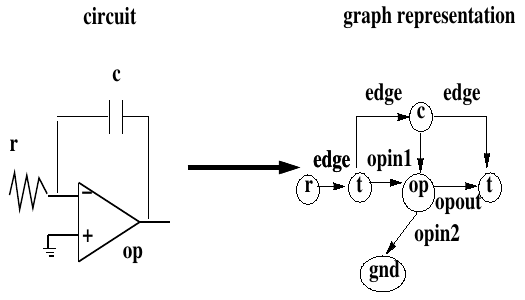
\includegraphics[width=0.9\textwidth,height=0.4\textheight,keepaspectratio]{electronics2.png} \\[-7pt]
      {\tiny Source: \cite{617051}}
    \end{column}
  \end{columns}
\end{frame}

\begin{frame}{Existing Ways to Solve It}
  \begin{itemize}
  \item \textsc{McSplit}, $\textsc{McSplit}{\downarrow}$
    \begin{itemize}
    \item \cite{DBLP:conf/ijcai/McCreeshPT17}
    \end{itemize}
  \item clique encoding
    \begin{itemize}
    \item \cite{DBLP:conf/cp/McCreeshNPS16}
    \end{itemize}
  \item $k{\downarrow}$
    \begin{itemize}
    \item \cite{DBLP:conf/aaai/HoffmannMR17}
    \end{itemize}
  \end{itemize}
\end{frame}

\begin{frame}{Solution: Algorithm Selection}
  \begin{figure}
    \centering
    \begin{tikzpicture}
      \node (graphs) at (0, 4) {$(G_1, G_2)$};
      \onslide<2->{\node (features) at (2, 4) {$\begin{bmatrix}f_1\\ \vdots \\ f_n\end{bmatrix}$};}
      \onslide<3->{\node[draw] (ml) at (5, 4) {ML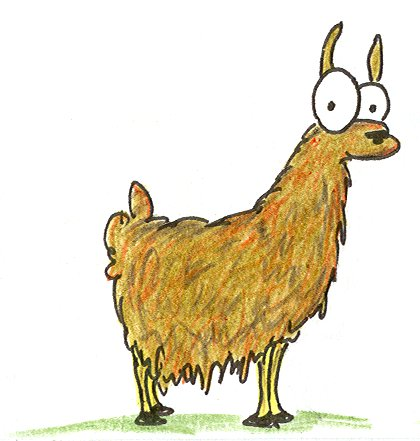
\includegraphics[scale=0.1]{llama.jpg}};}
      \onslide<4->{\node (mcsplit) at (2, 2) {\textsc{McSplit}};}
      \onslide<4->{\node (mcsplitdown) at (4, 2) {$\textsc{McSplit}{\downarrow}$};}
      \onslide<4->{\node (clique) at (6, 2) {clique};}
      \onslide<4->{\node (kdown) at (8, 2) {$k{\downarrow}$};}
      \onslide<6->{\node (answer) at (4, 0) {answer};}
      \path[->]<2-> (graphs) edge node[above] {\VarClock} (features);
      \path[->]<3-> (features) edge (ml);
      \path[->]<4-> (ml) edge (mcsplit);
      \only<1-4>{\tikzset{properties/.style={}}}
      \only<5->{\tikzset{properties/.style={ultra thick}}}
      \draw<4-> [->] (ml) edge[properties] (mcsplitdown);
      \path[->]<4-> (ml) edge (clique);
      \path[->]<4-> (ml) edge (kdown);
      \onslide<6->{\path[->] (mcsplitdown) edge node[right] {\VarClock} (answer);}
      \onslide<6->{\path[->]<6-> (graphs) edge [bend right=50] (4, 1);}
    \end{tikzpicture}
  \end{figure}
\end{frame}

\begin{frame}{The Process}
  \begin{itemize}
  \item Three cases:
    \begin{itemize}
    \item no labels
    \item vertex labels
    \item vertex and edge labels
    \end{itemize}
    \pause
  \item How many different labels?
    \begin{itemize}
    \item Measured as a percentage of the number of vertices/edges
    \item 5\%, 10\%, 15\%, 20\%, 25\%, 33\%, 50\%
    \end{itemize}
    \pause
  \item Run every algorithm on every instance
    \begin{itemize}
    \item $\sim\num{500000}$ experiments for each algorithm
    \end{itemize}
    \pause
  \item Identify and extract features
    \begin{itemize}
    \item 34 in total
    \item some from \cite{DBLP:conf/lion/KotthoffMS16}
    \item some new
    \end{itemize}
    \pause
  \item Train machine learning models
  \item Evaluate their performance and usefulness
  \end{itemize}
\end{frame}

%\begin{frame}{Features (34 in total)}
%  1--8 are from \cite{DBLP:conf/lion/KotthoffMS16}
%  \begin{enumerate}
%  \item number of vertices
%  \item number of edges
%  \item mean/max degree
%  \item density
%  \item mean/max distance between pairs of vertices
%  \item number of loops
%  \item proportion of vertex pairs with distance $\ge$ 2, 3, 4
%  \item connectedness
%    \pause
%  \item standard deviation of degrees
%  \item labelling percentage
%    \pause
%  \item ratios of features 1--5
%  \end{enumerate}
%\end{frame}

%\begin{frame}{Random forests \parencite{DBLP:journals/ml/Breiman01}}
%  \begin{figure}
%    \centering
%    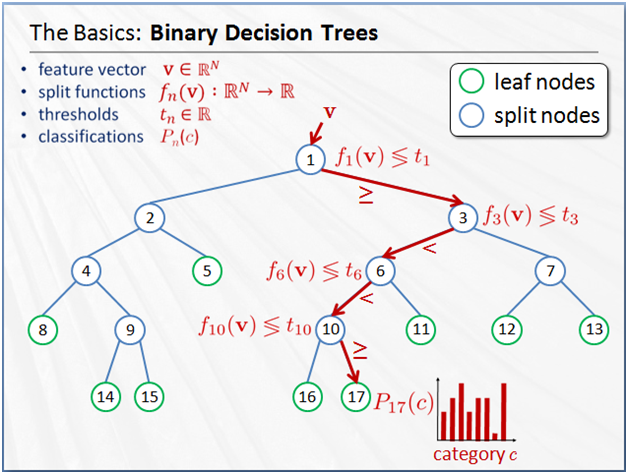
\includegraphics[scale=0.5]{random_forests_2.png} \\
%    {\tiny\color{gray}Source: Tae-Kyun Kim \& Bjorn Stenger, Intelligent Systems and Networks (ISN) Research Group,\\[-7pt] Imperial College London}
%  \end{figure}
%\end{frame}

%\begin{frame}{Random forests \parencite{DBLP:journals/ml/Breiman01}}
%  \begin{figure}
%    \centering
%    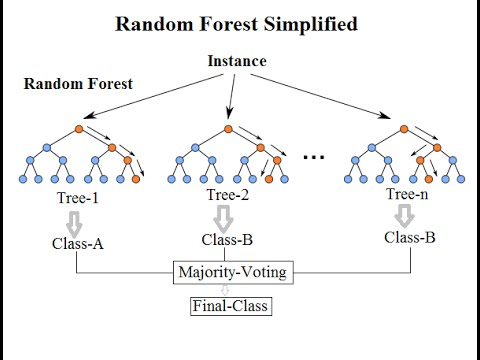
\includegraphics[scale=0.5]{rand-forest-1.jpg} \\
%    {\tiny\color{gray}Source: Random Forests(r), Explained, Ilan Reinstein, KDnuggets}
%  \end{figure}
%\end{frame}

\begin{frame}{Results}
  \begin{figure}
    \centering
    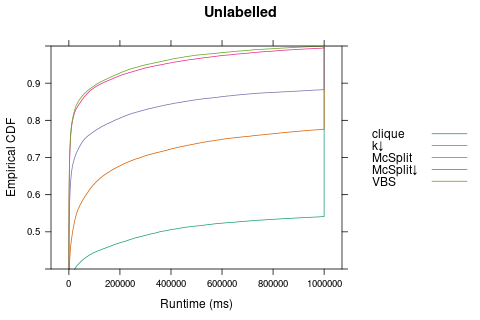
\includegraphics[width=\textwidth]{../dissertation/images/ecdf_unlabelled.png}
  \end{figure}
\end{frame}

\begin{frame}{Results (27\%)}
  \begin{figure}
    \centering
    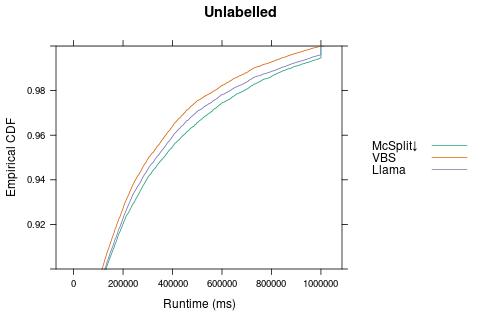
\includegraphics[width=\textwidth]{../dissertation/images/ecdf_unlabelled_llama.png}
  \end{figure}
\end{frame}

\begin{frame}{Results}
  \begin{figure}
    \centering
    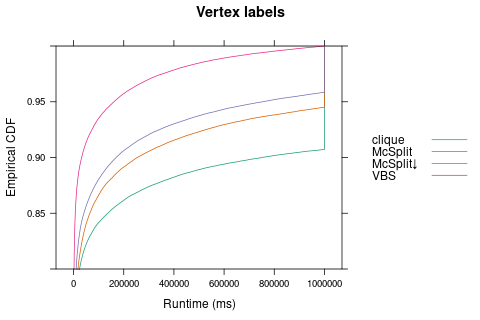
\includegraphics[width=\textwidth]{../dissertation/images/ecdf_vertex_labels.png}
  \end{figure}
\end{frame}

\begin{frame}{Results (86\%)}
  \begin{figure}
    \centering
    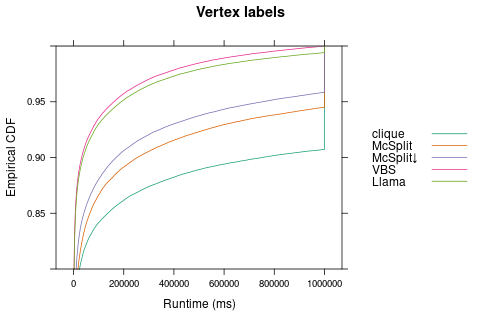
\includegraphics[width=\textwidth]{../dissertation/images/ecdf_vertex_labels_llama.png}
  \end{figure}
\end{frame}

\begin{frame}{Results}
  \begin{figure}
    \centering
    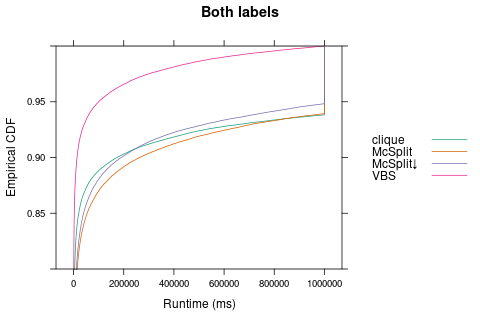
\includegraphics[width=\textwidth]{../dissertation/images/ecdf_both_labels.png}
  \end{figure}
\end{frame}

\begin{frame}{Results (88\%)}
  \begin{figure}
    \centering
    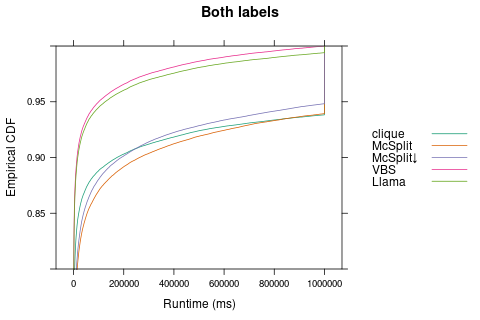
\includegraphics[width=\textwidth]{../dissertation/images/ecdf_both_labels_llama.png}
  \end{figure}
\end{frame}

%\begin{frame} % title?
%  \begin{columns}
%    \begin{column}{0.5\textwidth}
%      \begin{figure}
%        \centering
%        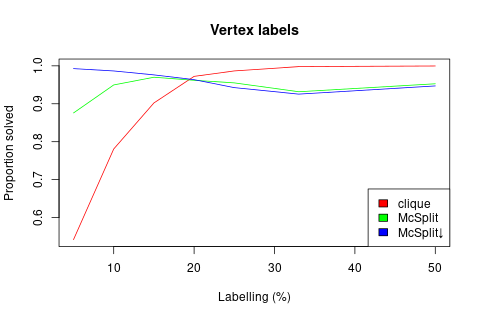
\includegraphics[width=\textwidth]{../dissertation/images/vertex_labels_linechart.png}
%        \visible<2>{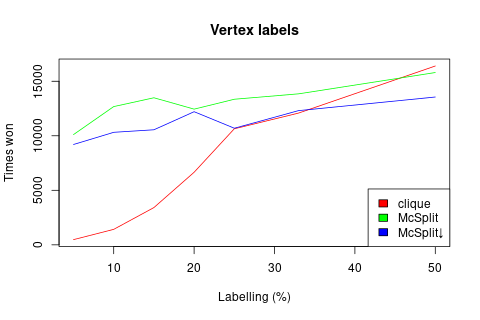
\includegraphics[width=\textwidth]{../dissertation/images/vertex_labels_linechart3.png}}
%      \end{figure}
%    \end{column}
%    \begin{column}{0.5\textwidth}
%      \begin{figure}
%        \centering
%        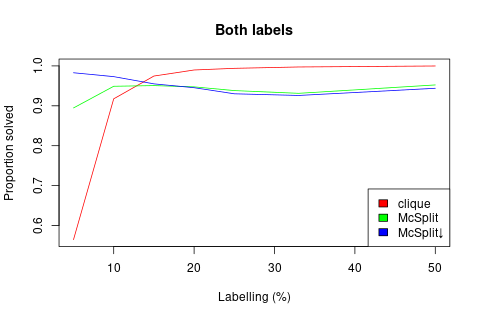
\includegraphics[width=\textwidth]{../dissertation/images/both_labels_linechart.png}
%        \visible<2>{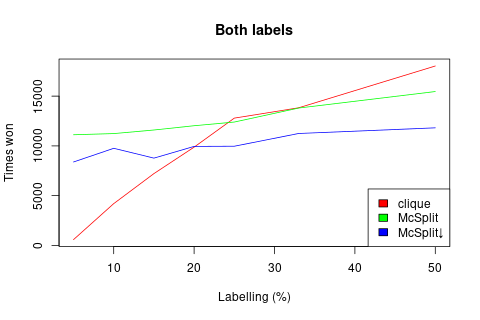
\includegraphics[width=\textwidth]{../dissertation/images/both_labels_linechart3.png}}
%      \end{figure}
%    \end{column}
%  \end{columns}
%\end{frame}

\begin{frame}{Other Accomplishments}
  \begin{itemize}
  \item Identified important features:
    \begin{itemize}
    \item labelling percentage, standard deviation of degrees
    \end{itemize}
  \item Discovered how algorithms' performance changes with fewer labels
  \item Extended $k{\downarrow}$ to support vertex labels
    \begin{itemize}
    \item using neighbourhood degree sequences
    \end{itemize}
  \item Defined and developed new algorithms capable of switching between
    \textsc{McSplit} and the clique encoding
  \end{itemize}
\end{frame}

\end{document}